  
\documentclass[journal,12pt,twocolumn]{IEEEtran}

\usepackage{setspace}
\usepackage{gensymb}
\singlespacing
\usepackage[cmex10]{amsmath}

\usepackage{amsthm}
\usepackage{commath}
\usepackage{mathrsfs}
\usepackage{txfonts}
\usepackage{stfloats}
\usepackage{bm}
\usepackage{cite}
\usepackage{cases}
\usepackage{subfig}
\usepackage{circuitikz}
\usepackage{longtable}
\usepackage{multirow}

\usepackage{enumitem}
\usepackage{mathtools}
\usepackage{steinmetz}
\usepackage{tikz}
\usepackage{circuitikz}
\usepackage{verbatim}
\usepackage{tfrupee}
\usepackage[breaklinks=true]{hyperref}
\usepackage{graphicx}
\usepackage{tkz-euclide}
\usepackage{array}
\usetikzlibrary{calc,math}
\usepackage{listings}
    \usepackage{color}                                            %%
    \usepackage{array}                                            %%
    \usepackage{longtable}                                        %%
    \usepackage{calc}                                             %%
    \usepackage{multirow}                                         %%
    \usepackage{hhline}                                           %%
    \usepackage{ifthen}                                           %%
    \usepackage{lscape}     
\usepackage{multicol}
\usepackage{chngcntr}

\DeclareMathOperator*{\Res}{Res}

\renewcommand\thesection{\arabic{section}}
\renewcommand\thesubsection{\thesection.\arabic{subsection}}
\renewcommand\thesubsubsection{\thesubsection.\arabic{subsubsection}}

\renewcommand\thesectiondis{\arabic{section}}
\renewcommand\thesubsectiondis{\thesectiondis.\arabic{subsection}}
\renewcommand\thesubsubsectiondis{\thesubsectiondis.\arabic{subsubsection}}
\newtheorem{theorem}{Theorem}[section]
\newtheorem{corollary}{Corollary}[theorem]
\newtheorem{lemma}[theorem]{Lemma}
\newtheorem{definition}{Definition}[section]

\hyphenation{op-tical net-works semi-conduc-tor}
\def\inputGnumericTable{}                                 %%

\lstset{
%language=C,
frame=single, 
breaklines=true,
columns=fullflexible
}
\begin{document}

\newcommand{\BEQA}{\begin{eqnarray}}
\newcommand{\EEQA}{\end{eqnarray}}
\newcommand{\define}{\stackrel{\triangle}{=}}
\bibliographystyle{IEEEtran}
\raggedbottom
\setlength{\parindent}{0pt}
\providecommand{\mbf}{\mathbf}
\providecommand{\pr}[1]{\ensuremath{\Pr\left(#1\right)}}
\providecommand{\qfunc}[1]{\ensuremath{Q\left(#1\right)}}
\providecommand{\sbrak}[1]{\ensuremath{{}\left[#1\right]}}
\providecommand{\lsbrak}[1]{\ensuremath{{}\left[#1\right.}}
\providecommand{\rsbrak}[1]{\ensuremath{{}\left.#1\right]}}
\providecommand{\brak}[1]{\ensuremath{\left(#1\right)}}
\providecommand{\lbrak}[1]{\ensuremath{\left(#1\right.}}
\providecommand{\rbrak}[1]{\ensuremath{\left.#1\right)}}
\providecommand{\cbrak}[1]{\ensuremath{\left\{#1\right\}}}
\providecommand{\lcbrak}[1]{\ensuremath{\left\{#1\right.}}
\providecommand{\rcbrak}[1]{\ensuremath{\left.#1\right\}}}
\theoremstyle{remark}
\newtheorem{rem}{Remark}
\newcommand{\sgn}{\mathop{\mathrm{sgn}}}
\providecommand{\abs}[1]{\vert#1\vert}
\providecommand{\res}[1]{\Res\displaylimits_{#1}} 
\providecommand{\norm}[1]{\lVert#1\rVert}
%\providecommand{\norm}[1]{\lVert#1\rVert}
\providecommand{\mtx}[1]{\mathbf{#1}}
\providecommand{\mean}[1]{E[ #1 ]}
\providecommand{\fourier}{\overset{\mathcal{F}}{ \rightleftharpoons}}
%\providecommand{\hilbert}{\overset{\mathcal{H}}{ \rightleftharpoons}}
\providecommand{\system}{\overset{\mathcal{H}}{ \longleftrightarrow}}
	%\newcommand{\solution}[2]{\textbf{Solution:}{#1}}
\newcommand{\solution}{\noindent \textbf{Solution: }}
\newcommand{\cosec}{\,\text{cosec}\,}
\providecommand{\dec}[2]{\ensuremath{\overset{#1}{\underset{#2}{\gtrless}}}}
\newcommand{\myvec}[1]{\ensuremath{\begin{pmatrix}#1\end{pmatrix}}}
\newcommand{\mydet}[1]{\ensuremath{\begin{vmatrix}#1\end{vmatrix}}}
\numberwithin{equation}{subsection}
\makeatletter
\@addtoreset{figure}{problem}
\makeatother
\let\StandardTheFigure\thefigure
\let\vec\mathbf
\renewcommand{\thefigure}{\theproblem}
\def\putbox#1#2#3{\makebox[0in][l]{\makebox[#1][l]{}\raisebox{\baselineskip}[0in][0in]{\raisebox{#2}[0in][0in]{#3}}}}
     \def\rightbox#1{\makebox[0in][r]{#1}}
     \def\centbox#1{\makebox[0in]{#1}}
     \def\topbox#1{\raisebox{-\baselineskip}[0in][0in]{#1}}
     \def\midbox#1{\raisebox{-0.5\baselineskip}[0in][0in]{#1}}
\vspace{3cm}
\title{Gate Assignment 3}
\author{Rongala Arun Siddardha - AI20BTECH11019}
\maketitle
\newpage
\bigskip
\renewcommand{\thefigure}{\theenumi}
\renewcommand{\thetable}{\theenumi}

%
Download latex-tikz codes from 
%
\begin{lstlisting}
https://github.com/ArunSiddardha/EE3900/blob/main/GATE_ASSIGNMENT_3/main.tex
\end{lstlisting}
\section{Problem(Gate EC 2004 Q.36)}
A system is described by the following differential equation
\begin{align}
    \frac{d^2y(t)}{dt^2}+3\frac{dy(t)}{dt}+2y(t) =x(t) \label{q}
\end{align}
is intially at rest.For the input $x\brak{t}=2u\brak{t}$ the output is given by
\begin{enumerate}
    \item $\brak{1-2e^{-t}+e^{-2t}}u\brak{t}$
    \item $\brak{1+2e^{-t}-e^{-2t}}u\brak{t}$
    \item $\brak{0.5+e^{-t}+1.5e^{-2t}}u\brak{t}$
    \item $\brak{0.5+2e^{-t}+2e^{-2t}}u\brak{t}$
\end{enumerate}
\section{Solution}
\begin{lemma}[Table of Laplace Transforms]\label{tbl}
\begin{center}
\begin{tabular}{ |m{3cm}|m{4.5cm}| } 
 \hline
 $\textbf{Time Function}$ $f(t)=\mathcal{L}^{-1}\cbrak{F(s)}$ & $\textbf{Laplace transform}$ of f(t) $F\brak{s}=\mathcal{L}\cbrak{f\brak{t}}$ \\ 
 \hline
 $u\brak{t}$ & $\frac{1}{s}$, $s>0$ \\ 
 \hline
 $g^{\prime}(t)$ & $sG\brak{s}-g(0)$ \\ 
 \hline
 $g^{\prime\prime}\brak{t}$ & $s^2G\brak{s}-sg\brak{0}-g^{\prime}\brak{0}$\\
 \hline
 $e^{-at}u\brak{t}$ & $\frac{1}{s+a}$, $s+a>0$\\
 \hline
\end{tabular}
\end{center}
\end{lemma}
\begin{lemma}{Linearity of Laplace Transform}
\begin{align}
    \mathcal{L}\cbrak{af\brak{t}+bg\brak{t}}=a\mathcal{L}\cbrak{f\brak{t}}+b\mathcal{L}\cbrak{g\brak{t}}
\end{align}
\end{lemma}
From Lemma-\ref{tbl} Laplace transform of $x\brak{t}=2u\brak{t}$ is given by
\begin{align}
    X\brak{s}=\frac{2}{s}
\end{align}
Since initialially it is at rest. Laplace Transform of $\eqref{q}$ gives
\begin{align}
    s^{2}Y\brak{s}+3sY\brak{s}+2Y\brak{s}&=X\brak{s}\\
    Y\brak{s}&=\frac{2}{s(s^2+3s+2)}\\
    = \frac{1}{s+2}+\frac{1}{s}+ \frac{-2}{s+1}\label{hc}\\
\end{align}
From Lemma-$\ref{tbl}$. Inverse Laplace transform of $Y\brak{s}$ is given by
\begin{align}
    y(t)&=-2e^{-t}u\brak{t}+e^{-2t}u\brak{t}+1 u\brak{t}\\
    &=\brak{-2e^{-t}+e^{-2t}+1}u\brak{t}
\end{align}
\begin{figure}[htp]
    \centering
    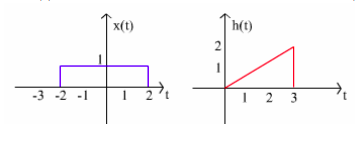
\includegraphics[width = \columnwidth]{fig1.png}
    \caption{Plot of input and output responses }
    \label{fig:my_label}
\end{figure}

$\therefore$ The required \textbf{option is A.}
\newpage
Building RLC circuit that satisfies $\eqref{q}$. Assume $\frac{R}{L}=3 $ and $LC=\frac{1}{2}$.
\begin{align}
  \text{Input}&:x\brak{t}\\
  \text{Output}&:y\brak{t}=V_1-V_0\label{f}
\end{align}
\begin{center}
\begin{circuitikz}[american voltages]
\draw (-4,0) to [american voltage source,l_=$x\brak{t}$](4,0);
\draw (-4,0) to (-4,3);
\draw (-4,3)to [L,l=$L$](-2,3) to [R,l=$R$](0,3) to [C,l=$C$](2,3) to [C,l=$C$](4,3);
\draw (2,3) to [short,l=$V_1$,-o](2,5);
\draw (4,3) to [short,l=$V_0$,-o](4,5);
\draw (4,0) to (4,3);
\end{circuitikz}
\end{center}
Using KVL laws
\begin{align}
 x\brak{t}-L\frac{di}{dt}-iR+\frac{2\int idt}{C}&=0\\
 V_1-V_0&=\frac{\int idt}{C} \label{l}
\end{align}
Eliminating $V_1,V_2,i$ from equations $\eqref{f}-\eqref{l}$ we get $\eqref{q}$. 
\begin{figure}[htp]
    \centering
    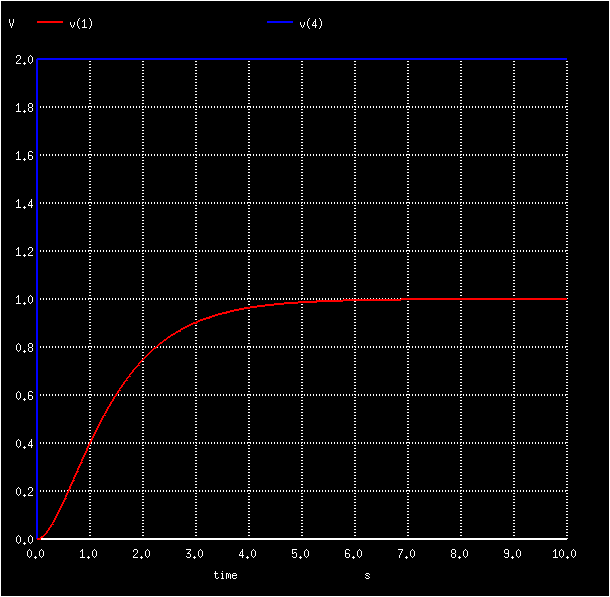
\includegraphics[width = \columnwidth]{fig.png}
    \caption{Plot obtained using ngspice input:blue and output:red }
    \label{fig:my_label}
\end{figure}
\end{document}
